\documentclass[]{exam}
\usepackage{epic,array,ecltree,url,calrsfs}
\usepackage[nointegrals]{wasysym}

%These tell TeX which packages to use.
\usepackage{array,epsfig}
\usepackage{amsmath}
\usepackage{amsfonts}
\usepackage{amssymb}
\usepackage{amsxtra}
\usepackage{amsthm}
\usepackage{mlextra} % must come after ams packages
\usepackage{mathrsfs}
\usepackage[dvipsnames]{xcolor}
\usepackage{array}
\usepackage{graphicx}
\graphicspath{ {../art/} }
\usepackage{subfig}
\usepackage{bm}
\usepackage{tikz}
\usepackage{multicol}
\usepackage{enumitem}

\newcommand{\twonode}{%
  \begingroup\normalfont
  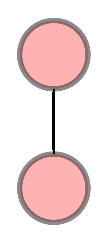
\includegraphics[height=\fontcharht\font`\b]{2nodetree.eps}%
  \endgroup
}

\newcommand{\tf}[1][{}]{%
\fillin[#1][0.25in]%
}
\title{Lab 8: Complexity, FOL, Prenex CNF}
\author{Foundations of Computer Science}
\date{\today}
%\pagestyle{empty} 
%\footer{}{\thepage}{}
\unframedsolutions
\SolutionEmphasis{\itshape\small}
\SolutionEmphasis{\color{NavyBlue}}


\begin{document}

\maketitle
\setlength{\columnseprule}{1pt}
\section*{Complexity}
\begin{questions} 
\question Recall Conway's Game of Life from the first lecture:
\url{https://bitstorm.org/gameoflife/}. Observe that as the game
progresses, each initial configuration leads inevitably to new
configurations. For example, State B in the figure below always
follows State A.
\begin{figure}[h]
\centering
\subfloat[State A]{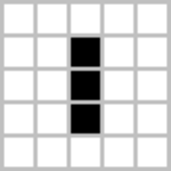
\includegraphics{GameoflifeblinkerA.pdf}}
\qquad
\subfloat[State B]{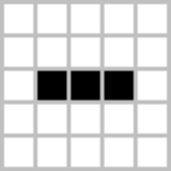
\includegraphics{GameoflifeblinkerB.pdf}}
\end{figure}
Consider the following general problem: given two states, $A$ and $B$, you
want to determine whether starting in state $A$ will eventually lead to
state $B$. In the following questions, we refer to this problem as
$\id{con-states}$.
\begin{parts}
\part A researcher writes a proof showing that every instance of the
$\id{con-states}$ problem can be translated into a statement in first order
logic that is valid if and only if State $A$ eventually leads to State
$B$. What can we conclude from this about the complexity of the 
$\id{con-states}$ problem?
\begin{solution}
~\\$\id{con-states} \leq \id{FOL-VAL}$. $\id{FOL-VAL}$ is semi-decidable, so
$\id{con-states}$ is also semi-deciable. 
\end{solution}
\part A second proof shows that any algorithm that could determine whether
an arbitrary statement in first order logic is satisfiable could also
be used to determine whether State $A$ eventually leads to State $B$ for any 
pair of states $A$ and $B$. Given both proofs, what can we say about the 
complexity of the $\id{con-states}$ problem?
\begin{solution}
~\\$\id{con-states} \leq \id{FOL-SAT}$. $\id{FOL-SAT}$ is neither decidable
nor semi-decidable, this gives us no new information about the complexity of
$\id{con-states}$.
\end{solution}
\part Finally, a third proof presents the following argument: Conway's Game
of life can simulate the behavior of an arbitrary Turing machine by
encoding the machine and its input as some configuration of the board. The proof
shows how this can be done and demonstrates that the progress of the game
under these circumstances corresponds exactly to the behavior of the machine.
Furthermore, the proof shows that under these assumptions there is a state of
the board that corresponds to a Turing machine that can make no further moves. 
Assuming this is convincingly demonstrated, and taking the
two previous proofs into account, what can we conclude
about the complexity of the $\id{con-states}$ problem?
\begin{solution}
~\\Since we can assign state $A$ to any initial state of the Turing machine and
state $B$ to a halted state, the solution to $\id{con-states}$ would allow us
to determine whether an arbitrary Turing machine halts on a given input.
Therefore, $\id{HALT} \leq \id{con-states}$. Since $\id{HALT}$ is undecidable
$\id{con-states}$ is undecidable. We know from previous results that it is
also semi-decidable.
\end{solution}
\end{parts}
\clearpage

\uplevel{\section*{First Order Logic}}

\question Consider the following interpretation $\mathcal{I} = (P,\{L,H\},\{\})$,
where $P$ is a set of people, $L$ is a unary relation such that $L(x)$ if and
only if $x$ is a librarian, and $H$ is a unary relation such that $H(x)$ if
and only if $x$ is happy. Write a statement in first order logic to express
the following:
\begin{parts}
\part All librarians are happy if only librarians are happy.
\begin{solution}
$\forall x ((\ngg L(x) \imp \ngg H(x)) \imp (L(x) \imp H(x)))$
\end{solution}

\part If it is the case that if someone is a librarian, no one is happy, then
no librarian is happy.
\begin{solution}
$(\exists x L(x) \imp \forall y \ngg H(y)) \imp \forall x(L(x) \imp \ngg H(x))$
\end{solution}

\end{parts}



\question Transform each of the following formulas to prenex normal form:
\begin{parts}
\part $\forall x(p(x) \imp \exists y q(y))$
\begin{solution}
~\\
\begin{tabular}{ll}
\text{Original formula:} & $\forall x (p(x) \imp \exists y q(y))$\\
\text{Simplify Boolean Operators:} & $\forall x (\ngg p(x) \lor \exists y q(y))$\\
\text{Extract quantifiers:} & $\forall x \exists y (\ngg p(x) \lor q(y))$
\end{tabular}
\end{solution}
\part $\forall x \forall y (\exists z p(z) \land \exists u (q(x,u) \imp \exists v q(y,v)))$
\begin{solution}
~\\
\begin{tabular}{ll}
\text{Original formula:} & $\forall x \forall y (\exists z p(z) \land \exists u
    (q(x,u) \imp \exists v q(y,v)))$\\
\text{Simplify Boolean Operators:} & $\forall x \forall y (\exists z p(z) \land
    \exists u (\ngg q(x,u) \lor \exists v q(y,v)))$\\
\text{Extract quantifiers:} & $\forall x \forall y \exists z \exists u \exists v (p(z) \land (\ngg q(x,u) \lor q(y,v)))$
\end{tabular}
\end{solution}
\part $\exists x(\ngg \exists yp(y) \imp \exists z(q(z) \imp r(x))$
\begin{solution}
~\\
\begin{tabular}{ll}
\text{Original formula:} & $\exists x(\ngg \exists yp(y) \imp \exists z(q(z) \imp r(x))$\\
\text{Simplify Boolean Operators:} & $\exists x(\ngg \ngg \exists yp(y) \lor \exists z(\ngg q(z) \lor r(x))$\\
\text{Push negation inwards:} & $\exists x(\exists yp(y) \lor \exists z(\ngg q(z) \lor r(x))$\\
\text{Extract quantifiers:} & $\exists x \exists y \exists z (p(y) \lor \ngg q(z) \lor r(x))$\\
\end{tabular}
\end{solution}
\end{parts}

\end{questions}
\end{document}


